\input{Catfying_zxCalc--Preamble}

%%%%%%%%%%%%%%%
%%%%%%%%%%%%%%%
\begin{document}
%%%%%%%%%%%%%%%
%%%%%%%%%%%%%%%

% FRAME ------------------

\begin{frame}{Compositionality}
	What is it?
	
	\pause
	
	A method to study a complex system
	by studying its component pieces
	and their connections.
	
	% put in an image of black boxing or something
	
\end{frame}{Compositionality}

% FRAME ------------------

\begin{frame}
	
	Examples of compositionality ...
	
	\pause
	
	a discussion of quantum teleportation in
	Abramsky \& Coecke's 
	\emph{A categorical semantics of quantum protocols}
	
	\includegraphics{QuantumTeleportation}
	
\end{frame}

% FRAME ------------------

\begin{frame}{Compositionality}
	Examples of compositionality ...
	
	\pause
	
	defining open Markov processes
	in Baez, Fong, \& Pollard's
	\emph{A compositional framework
	for Markov processes}
	
	\includegraphics{PetriNetComposition}
\end{frame}

% FRAME ------------------

\begin{frame}{Compositionality}
	Examples of compositionality ...
	
	\pause
	
	modeling open systems with Petri nets
	in Sassone \& Soboci\'{n}ski's
	\emph{A congruence for Petri nets}
	
	% stick a picture from the paper in here
	
\end{frame}

% FRAME ------------------

\begin{frame}{Compositionality}
	
	Common features include
	
	\pause
	
	open diagrams,
	i.e. \emph{mathematical gadgets
	with inputs and outputs}
	
	\pause 
	
	and
	
	equality given by symmetric rewrite rules,
	i.e. \emph{diagrams $D$ and $D'$ are equal
	if $D$ rewrites to $D'$ and $D'$ rewrites to $D$}

\end{frame}

% FRAME ------------------

\begin{frame}
	
	question
	
	Is there a general framework
	in which to place systems describable with
	open diagrams and rewriting?
	
\end{frame}

% FRAME ------------------

\begin{frame}{Modeling open systems}
	
	Let $G$ be an algebraic gadget,
	for instance a directed graph.
	
	\pause
	
	Let $I$ and $O$ be sub-gadgets
	that play the role of the 
	inputs and outputs for $G$.
	
	\pause
	
	Capture this system with a cospan
	\[
		I \to G \gets O
	\]
	 whose arrows are the appropriate morphisms.
	 
	 \pause
	 
	 In this way, we model suitable open systems
	 with cospans.
	 
\end{frame}

% FRAME ------------------

\begin{frame}{Modeling rewrite rules}
	
	As long as we are working within an
	adhesive category, we can
	model rewrite rules using the 
	\emph{double pushout} approach.
	
	\pause
	
	That is, a rewrite rule is a span of gadgets:
	\[
	L \gets K \to R
	\]
	reads as `$L$ rewrites to $R$'. 
	
\end{frame}

% FRAME ------------------

\begin{frame}{Combining open systems and rewriting}
	
	How can we rewrite an open system?
	
	\pause
	
	Use \emph{spans of cospans}:
	
	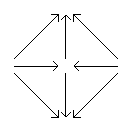
\includegraphics{diagram_span_cospans}
	
	\emph{(Note: Kissinger considered these
		in "Pictures of processes")}
		
\end{frame}

% FRAME ------------------

\begin{frame}{Combining open systems and rewriting}
	
	The components we are working with are:
	
	\begin{itemize}
		\item inputs and outputs modeled by a suitable gadget,
		\item open systems modeled by a cospan of gadgets,
		\item rewrites of open systems modeled by a span of cospans of gadgets.
	\end{itemize}
	
	\pause
	
	This list seems bicategorical. Is it?
	
\end{frame}

% FRAME ------------------

\begin{frame}
	
\end{frame}

% FRAME ------------------

\begin{frame}
	
\end{frame}

% FRAME ------------------

\begin{frame}
	
\end{frame}

% FRAME ------------------

\begin{frame}
	
\end{frame}

% FRAME ------------------

\begin{frame}
	
\end{frame}

% FRAME ------------------

\begin{frame}
	
\end{frame}

% FRAME ------------------

\begin{frame}
	
\end{frame}

\end{document}
